\subsection{格栅}
\subsubsection{基础数据}
\begin{enumerate}
	\item 污水平均日流量$Q$:
	$$Q=35000\;\text{m$^3$/d}=35000\times\dfrac{1000}{24\times60\times60}\;\text{L/s}=\eval{35000\times\dfrac{1000}{24\times60\times60}}[3]\;\text{L/s}$$
	\item 生活污水量总变化系数$K_z$:
	
	查阅《室外排水设计标准》(GB 50014-2021)可得到综合生活污水量变化系数表如下:
	\begin{table}[H]
		\centering
		\caption{综合生活污水量变化系数\cite{GB500152019}}
		\begin{tabular}{ccccccccc}
		\toprule
		平均日流量(L/s) & 5     & 15    & 40    & 70    & 100   & 200   & 500   & $\geqslant 1000$ \\
		\midrule
		变化系数  & 2.7   & 2.4   & 2.1   & 2.0     & 1.9   & 1.8   & 1.6   & 1.5 \\
		\bottomrule
		\multicolumn{9}{l}{注:当污水平均日流量为中间数值时,变化系数可用内插法求得。} \\
		\end{tabular}
		\label{tab:Comprehensive domestic sewage volume change coefficient}
	\end{table}

	因为污水平均日流量$Q=405.093\;\text{L/s}$,处于$200\;\text{L/s}\sim 500\;\text{L/s}$之间,则可以使用内插法求得:

	\begin{equation}
		\dfrac{Q-200}{K_z-1.8}=\dfrac{500-200}{1.6-1.8}
	\end{equation}
	\begin{align*}
		\therefore K_z=\dfrac{1.6-1.8}{500-200}(Q-200)+1.8 &=\dfrac{1.6-1.8}{500-200}\times(405.093-200)+1.8 \\
		&=\eval{\dfrac{1.6-1.8}{500-200}\times(405.093-200)+1.8}[2]
	\end{align*}

	\item 设计最大流量$Q_{max}$:
	$$Q_{max}=K_zQ=\workKz\times 35000\;\text{m$^3$/d}=58100 \;\text{m$^3$/d}=\eval{35000\times\dfrac{1}{24\times60\times60}\times1.66}[3]\;\text{m$^3$/s}$$
\end{enumerate}

\subsubsection{粗格栅计算草图}
粗格栅的主要功能是通过物理筛选的方式将污水中的大块固体物质、悬浮物、杂草、沙子等较大的颗粒物拦截下来,以防止它们进入后续的处理单元,从而减少对系统的损坏和故障的影响。

% 本次设计粗格栅由一组格栅宽度为 193 mm 的金属栅条与金属框架组成,其中栅条宽度为 $S=10$ mm,进水渠宽 $B_1=1.26$ m,格栅与水平面夹角 $\alpha$ 为60°,如下图所示:

\vskip2em

\begin{figure}[H]
	\centering
	% 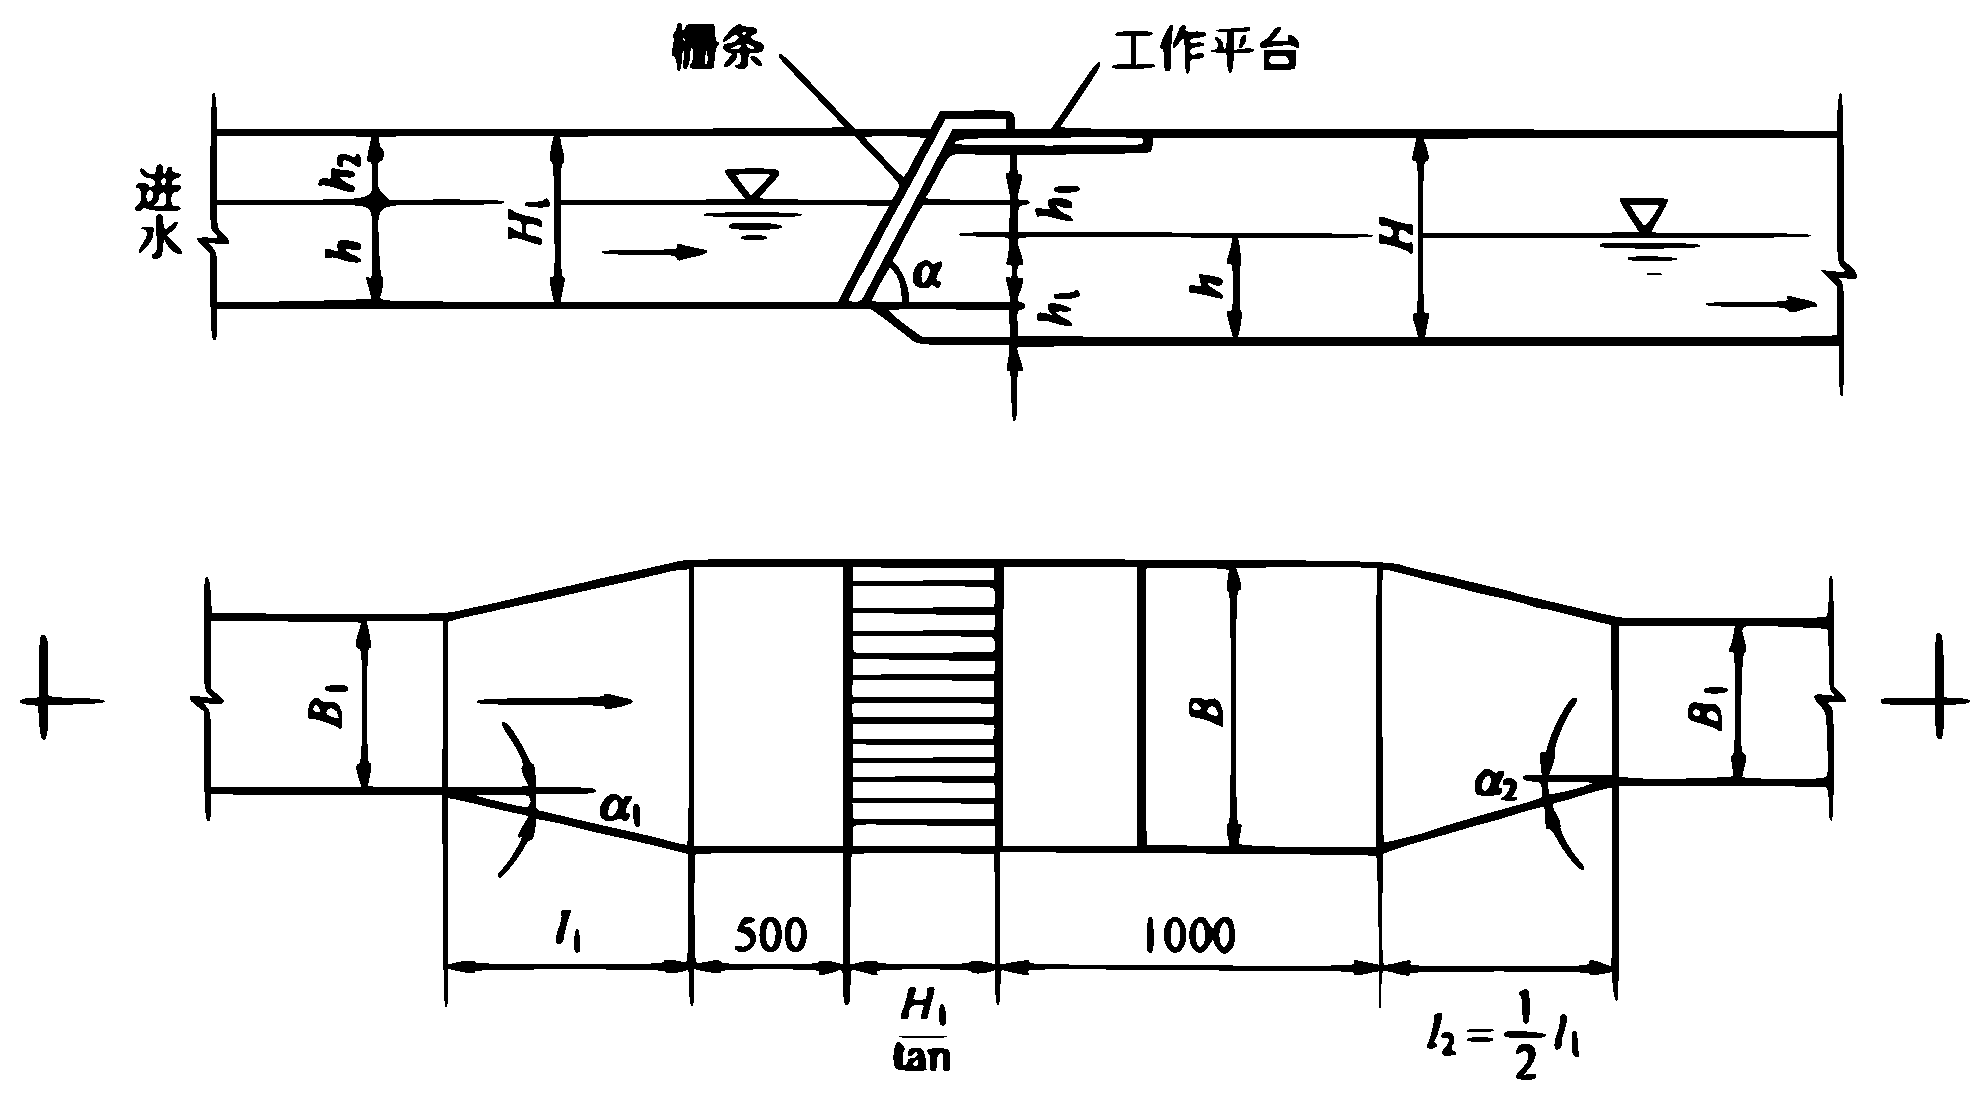
\includegraphics[width=\textwidth]{figures/Coarse-grille-sketch.pdf}
	\begin{subfigure}[htbp]{\textwidth}
		\centering
		\begin{tikzpicture}[scale=0.8]
			% 画折断线
			\draw (0,-0.5) -- ++(0,1) -- ++(-0.2,0.2) -- ++(0.4,0) -- ++(-0.2,0.2) -- (0,2.5);
			\draw (16,-1) -- ++(0,1) -- ++(-0.2,0.2) -- ++(0.4,0) -- ++(-0.2,0.2) -- (16,2.5);
			\node[left] at (-0.3,1) {进水};
			\node[right] at (16.3,1) {\phantom{进水}};
			% 画主体
			\draw (0,2) -- ++(16cm,0);
			\draw (0,1.2) -- ++(8cm,0);
			\draw (7.5,0.7) -- (16,0.7);
			\draw (0,0) -- ++(8cm,0);
			\draw (16,-0.5) -- ++(-9cm,0) -- ++(-0.5,0.5);
			% 画工作平台
			\draw (8,2) -- ++(2,0) -- ++(0,-0.2) -- ++(-2,0) -- cycle;
			\draw (8.8,2) -- ++(1,1) node[right] {工作平台};
			% 标记符号
			\draw (6.3,0) ++(0.5,0) arc (0:60:0.5) node[midway, right] {$\alpha$};
			\draw[stealth-stealth] (1.5,0) -- (1.5,1.2) node[midway, left] {$h$};
			\draw[stealth-stealth] (1.5,1.2) -- (1.5,2) node[midway, left] {$h_2$};
			\draw[stealth-stealth] (3,0) -- (3,2) node[midway, below left] {$H_1$};
			\draw[stealth-stealth] (8,-0.5) -- ++(0,0.5) node[right] {$h_1$};
			\draw[stealth-stealth] (8,0.7) -- ++(0,0.5) node[right] {$h_1$};
			\draw[stealth-stealth] (10,-0.5) -- ++(0,1.2) node[midway, left] {$h$};
			\draw[stealth-stealth] (12,-0.5) -- ++(0,2.5) node[midway, above left] {$H$};
			% 画格栅
			\draw (7.4,1.5) -- ++(-1.5,1.5) node[left] {格栅};
			\draw[fill=white] (8,2) -- ++(0.6,0) -- ++(0,0.15) -- ++(-0.65,0) -- (6,0) -- ++(0.2,0) -- cycle;
			% 画标识
			\draw[-stealth, line width=1.2pt] (3.5,0.6) -- ++(1,0);
			\draw[-stealth, line width=1.2pt] (14.5,0.1) -- ++(1,0);
			\foreach \x/\y in {5/1.2, 14/0.7} {
				\draw (\x,\y) -- ++(-0.3,0.3) -- ++(0.6,0) --cycle;
				\draw (\x,\y) ++(-0.5,-0.1) -- ++(1,0);
				\draw (\x,\y) ++(-0.3,-0.2) -- ++(0.6,0);
				\draw (\x,\y) ++(-0.1,-0.3) -- ++(0.2,0);
			}
		\end{tikzpicture}
		\caption{正视图}
	\end{subfigure}

	\begin{subfigure}[htbp]{\textwidth}
		\centering
		\begin{tikzpicture}[scale=0.8]
			% 画对称线
			\draw (-2,1) ++(-0.5,0) -- ++(1.5,0);
			\draw (-2,1) ++(0,-0.5) -- ++(0,1.5);
			\draw (18,1) ++(-1,0) -- ++(1.5,0);
			\draw (18,1) ++(0,-0.5) -- ++(0,1.5);
			% 画折断线
			\draw (0,-0.5) -- ++(0,1.3) -- ++(-0.2,0.2) -- ++(0.4,0) -- ++(-0.2,0.2) -- (0,2.5);
			\draw (16,-0.5) -- ++(0,1.3) -- ++(-0.2,0.2) -- ++(0.4,0) -- ++(-0.2,0.2) -- (16,2.5);
			% 画主体
			\foreach \d in {0.6} {
				\draw (0,0) -- ++(1.5,0) -- ++(2.5,-\d)-- ++(8,0) -- ++(2.5,\d) -- ++(1.5,0);
				\draw (0,2) -- ++(1.5,0) -- ++(2.5,\d)-- ++(8,0) -- ++(2.5,-\d) -- ++(1.5,0);
				\foreach \x in {1.5,14.5} {
					\draw (\x,0) -- ++(0,2);
				}
				\foreach \x in {4,6,8,9.5,12} {
					\draw (\x,-\d) -- ++(0,2+2*\d);
				}
				\foreach \y in {0,0.1,...,1} {
					\draw (6,{\y*(2+2*\d)-\d}) -- ++(2,0);
				}
				% 画标注
				\foreach \y in {1.2} {
					\draw (1.5,0) -- ++(0,-\y-\d);
					\draw (14.5,0) -- ++(0,-\y-\d);
					\foreach \x in {4,6,8,12} {
						\draw (\x,-\d) -- ++(0,-\y);
					}
					\draw[stealth-stealth] (1.5,0.2-\y-\d) -- ++(2.5,0) node[midway, above] {$l_1$};
					\draw[stealth-stealth] (14.5,0.2-\y-\d) -- ++(-2.5,0) node[midway, below] {$l_2=\dfrac{1}{2}l_1$};
					\draw[stealth-stealth] (4,0.2-\y-\d) -- ++(2,0) node[midway, above] {$500$};
					\draw[stealth-stealth] (6,0.2-\y-\d) -- ++(2,0) node[midway, below] {$\dfrac{H_1}{\tan{\alpha}}$};
					\draw[stealth-stealth] (8,0.2-\y-\d) -- ++(4,0) node[midway, above] {$1000$};
				}
				\foreach \x in {1,15.5} {
					\draw[stealth-stealth] (\x,0) -- ++(0,2) node[midway, left] {$B_1$};
				}
				\draw[stealth-stealth] (10.5,-\d) -- ++(0,{2+2*\d}) node[midway, left] {$B$};
				\draw[-stealth, line width=1.2pt] (2,1) -- ++(1.5,0);
				% 画角度
				\draw (3.5,0) -- ++(-2,0) ++(1.5,0) arc (0:-{atan(\d/2.5)}:1.5cm) node[midway, right] {$\alpha_1$};
				\draw (12.5,0) -- ++(2,0) ++(-1.5,0) arc (180:{180+atan(\d/2.5)}:1.5cm) node[midway, left] {$\alpha_2$};
			}
		\end{tikzpicture}
		\caption{俯视图}
	\end{subfigure}

	\caption{粗格栅计算草图}
	\label{fig:Coarse grille sketch}
\end{figure}


\subsubsection{粗格栅的计算}
一般格栅的计算理论主要是以平面格栅为研究对象,对于曲面格栅应考虑折减和换算。在进行工程设计和格栅选型时,应在格栅理论计算的基础上,结合工程设计实际和选型格栅特点统筹考虑。查阅张辰主编的《污水厂设计》得到格栅设计相关计算公式如下:

\footnotesize
\begin{longtable}{l|l|l}
	\caption{格栅设计计算公式\cite[p.114]{《污水厂设计》}}\label{tab:Grille design calculation formula} \\
	\toprule
	名称    & 公式    & 符号说明 \\
	\midrule
	\endfirsthead
	
	\multicolumn{3}{c}%
	{{\tablename\ \thetable{} -- 续表}} \\
	\toprule
	名称    & 公式    & 符号说明 \\
	\midrule
	\endhead
	
	\bottomrule
	\endfoot
	
	\bottomrule
	\endlastfoot
	
	栅槽宽度 & \makecell[l]{$B=S(n-1)+bn+0.2$\\ $n =\dfrac{Q_{max}\sqrt{\sin\alpha}}{bhv}$} & \makecell[l]{$B$——栅槽宽度,m;\\
	$S$——栅条宽度,m;\\
	$b$——栅条间隙,m;\\
	$n$——栅条间隙数,个;\\
	$Q_{max}$——最大设计流量,m$^3$/s;\\
	$\alpha$——格栅倾角,度;\\
	$h$——栅前水深,m;\\
	$v$——过栅流速,m/s} \\
	
	\midrule
	通过格栅的水头损失 & \makecell[l]{$h_1=h_0k$\\ $h_0=\xi\dfrac{v^2}{2g}\sin\alpha$} & \makecell[l]{$h_1$——通过格栅的水头损失,m;\\
	$h_0$——计算水头损失,m;\\
	$g$——重力加速度,m/s$^2$;\\
	$k$——系数,格栅受污物堵塞时水头损失增大倍数,\\
	\phantom{$k$——}一般采用3;\\
	$\xi$——阻力系数,其值与栅条断面形状有关,\\
	\phantom{$\xi$——}可按表 \ref{tab:The drag coefficient xi calculation formula} 计算} \\
	
	\midrule
	栅后槽总高度  & $H=h+h_1+h_2$   & \makecell[l]{$H$——栅后槽总高度,m;\\
	$h_2$——栅前渠道超高,一般采用 0.3 m} \\
	
	\midrule
	栅槽总长度  &  \makecell[l]{$L=l_1+l_2+1.0+0.5+\dfrac{H_1}{\tan\alpha}$\\ $l_1=\dfrac{B-B_1}{2\tan\alpha_1}$\\ $l_2=\dfrac{l_1}{2}$\\ $H_1=h+h_2$}   & \makecell[l]{$L$——栅槽总长度,m;\\
	$l_1$——进水渠道渐宽部分的长度,m;\\
	$B_1$——进水渠宽,m;\\
	$\alpha_1$——进水渠道渐宽部分的展开角度,一般可采用20°;\\
	$l_2$——栅渣与出水渠道连接处的渐窄部分长度,m;\\
	$H_1$——栅前渠道深,m} \\
	
	\midrule
	每日栅渣量 & \makecell[l]{$W=\dfrac{Q_{max}W_1\times86400}{K_z\times1000}$} &  \makecell[l]{$W$——每日栅渣量,m$^3$/d;\\
	$W_1$——单位栅渣量,m$^3$/10$^3$m$^3$ 污水;\\
	格栅间隙为 $16\sim 25$ mm时,$W_1=0.10\sim 0.05$;\\
	格栅间隙为 $30\sim 50$ mm时,$W_1=0.03\sim 0.01$;\\
	$K_z$——生活污水流量总变化系数} \\
\end{longtable}
\normalsize

\begin{table}[H]
	\centering
	\caption{阻力系数 $\xi$ 计算公式\cite[p.114]{《污水厂设计》}}
	\begin{tabular}{l|l|l}
		\toprule
		棚条断面形状    & 公式    & 说明 \\
		\midrule
		\makecell[l]{\null\\锐边矩形\\迎水面为半圆形的矩形\\圆形\\迎水、背水面均为半圆形的矩形} & $\xi=\beta\left(\dfrac{S}{b}\right)^{\frac{4}{3}}$ & \makecell[l]{形状系数\\ $\beta=2.42$\\ $\beta=1.83$\\ $\beta=1.79$\\ $\beta=1.67$} \\
		\midrule
		正方形 & $\xi=\left(\dfrac{b+S}{\varepsilon b}-1\right)^{2}$ & \makecell[l]{$\varepsilon$——收缩系数,一般采用0.64} \\
		\bottomrule
	\end{tabular}%
	\label{tab:The drag coefficient xi calculation formula}%
\end{table}%


\begin{enumerate}
	\item 栅槽宽度
	
	\begin{enumerate}
		\item 栅前水深、进水渠宽:
		
		水力最优梯形断面宽深比\cite{水力最优——《水力学》第六章}:
		\begin{equation}
			\beta = \dfrac{b}{h} =2\left(\sqrt{1+m^2}-m\right)
		\end{equation}
		$b$——进水渠宽,m;\par
		$h$——栅前水深,m;\par
		$m$——边坡系数。
		
		因为进水渠形状设计为矩形,如下图 \ref{fig:Sketch of the shape of the intake canal} 所示:
		\begin{figure}[H]
			\centering
			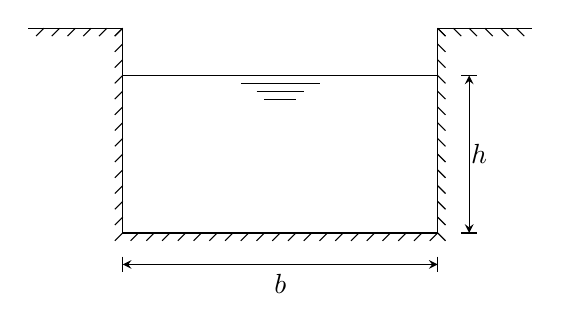
\begin{tikzpicture}
				\draw (-1.2,2.6) -- (0,2.6) -- (0,0) -- (4,0) -- (4,2.6) -- (5.2,2.6);
				\foreach \x in {0,0.2,...,4} % 绘制地面上的刻度线
					\draw (\x,0) -- (\x-0.1,-0.1);
				\foreach \x in {-1,-0.8,...,0} % 绘制地面上的刻度线
					\draw (\x,2.6) -- (\x-0.1,2.5);
				\foreach \x in {4,4.2,...,5} % 绘制地面上的刻度线
					\draw (\x,2.6) -- (\x+0.1,2.5);
				\foreach \y in {0.2,0.4,...,2.6} % 绘制地面上的刻度线
					\draw (0,\y) -- (-0.1,\y-0.1);
				\foreach \y in {0,0.2,...,2.6} % 绘制地面上的刻度线
					\draw (4,\y) -- (4.1,\y-0.1);

				\draw (0,2) -- (4,2); % 水面高度
				\draw (2,2) ++(-0.5,-0.1) -- ++(1,0);
				\draw (2,2) ++(-0.3,-0.2) -- ++(0.6,0);
				\draw (2,2) ++(-0.2,-0.3) -- ++(0.4,0);
			
				\foreach \x in {0,2}
					\draw (4.3,\x) -- (4.5,\x);
				\draw[stealth-stealth] (4.4,0) -- (4.4,2);
				\node[right] at (4.3,1) {$h$};
				\foreach \x in {0,4}
					\draw (\x,-0.3) -- (\x,-0.5);
				\draw[stealth-stealth] (0,-0.4) -- (4,-0.4);
				\node[below] at (2,-0.4) {$b$};
			\end{tikzpicture}
			\caption{进水渠形状草图}
			\label{fig:Sketch of the shape of the intake canal}
		\end{figure}
		则易知边坡系数 $m=0$ ,所以
		\begin{equation*}
			\beta = \dfrac{b}{h} =2\left(\sqrt{1+0^2}-0\right) = 2
		\end{equation*}
		即
		\begin{equation}
			b=2h
		\end{equation}

		明渠均匀流基本公式\cite{水力最优——《水力学》第六章}:
		\begin{equation}
			Q=Av
		\end{equation}
		$Q$——流量,m$^3$;\par
		$A$——截面面积,m$^2$;\par
		$v$——流速,m/s。取 $v=0.85$ m/s\footnote{《室外排水设计标准》(GB 50014-2021):污水过栅流速宜采用 0.6 m/s $\sim$ 1.0 m/s。}。

		又因为进水渠的截面面积为
		\begin{equation}
			A=bh
		\end{equation}

		所以当流量为设计最大流量 $Q_{max}=0.672$ m$^3$/s 时,将上述公式联立求解,可得到每台格栅机栅前水深 $h$、进水渠宽 $B_1$:
		\begin{align*}
			B_1=b=\sqrt{\dfrac{2Q_{max}}{v}}=\sqrt{\dfrac{2\times0.672}{0.85\times2}} \;\text{m} =\eval{\sqrt{\dfrac{2\times0.672}{0.85\times2}}}[2] \;\text{m} \\
			h=h=\sqrt{\dfrac{Q_{max}}{2v}}=\sqrt{\dfrac{0.672}{2\times 0.85\times2}} \;\text{m} = \eval{\sqrt{\dfrac{0.672}{2\times 0.85\times2}}}[2] \;\text{m}
		\end{align*}
		\item 栅条的间隙数:
		
		因为格栅选择的是机械清除,所以取 $b=0.021$ m\footnote{《室外排水设计标准》(GB 50014-2021)粗格栅栅条间隙宽度规定:机械清除时宜为16 mm $\sim$ 25 mm,人工清除时宜为25 mm $\sim$ 40 mm,特殊情况下,最大间隙可为100 mm。},
		取 $\alpha=60$°\footnote{《室外排水设计标准》(GB 50014-2021):除转鼓式格栅除污机外,机械清除格栅的安装角度宜为 60°$\sim$90°。},
		共有2台格栅机器,则每台格栅机器的栅槽宽度为
		\begin{align}
			n =\dfrac{Q_{max}\sqrt{\sin\alpha}}{bhv}&=\dfrac{\dfrac{0.672}{2}\times\sqrt{\sin{\dfrac{\pi}{3}}}}{0.021\times0.44\times0.85}=\eval{\dfrac{\frac{0.672}{2}\times\sqrt{\sin{\frac{\pi}{3}}}}{0.021\times0.44\times0.85}}[1] \;\text{(条)}\\
			&\approx 40\;\text{(条,向上取整)} \notag
		\end{align}
		
		\item 栅槽宽度:

		因为栅条宽度 $S=0.01$ m,则
		\begin{align}
			B=S(n-1)+bn+0.2 &=0.01\times(40-1)+0.021\times40+0.2 \;\text{m} \\
			&=\eval{0.01\times(40\times 2-1)+0.021\times40+0.2}[2]\;\text{m} \notag
		\end{align}
	\end{enumerate}
	
	\item 通过格栅的水头损失
	
	\begin{enumerate}
		\item 计算水头损失:

		因为栅条断面形状为锐边矩形,由表 \ref{tab:The drag coefficient xi calculation formula} 可知$\beta=2.42$,则
		\begin{align}
			\xi=\beta\left(\dfrac{S}{b}\right)^{\frac{4}{3}} =2.42\times\left(\dfrac{0.01}{0.021}\right)^{\frac{4}{3}}=\eval{2.42\times\left(\dfrac{0.01}{0.021}\right)^{\frac{4}{3}}}[3] 
		\end{align}

		又因为重力加速度 $g=9.8$ m/s$^2$,则
		\begin{align}
			h_0=\xi\dfrac{v^2}{2g}\sin\alpha=0.9\times\dfrac{0.85^2}{2\times9.8}\sin{\frac{\pi}{3}}\;\text{m}=\eval{0.9\times\dfrac{0.85^2}{2\times9.8}\sin{\frac{\pi}{3}}}[4] \;\text{m}
		\end{align}

		\item 通过格栅的水头损失:

		取 $k=3$\footnote{由表 \ref{tab:Grille design calculation formula} 可知,系数 $k$,格栅受污物堵塞时水头损失增大倍数,一般采用3。},则
		\begin{align}
			h_1=h_0k=0.0287\times3 \;\text{m}=\eval{0.9\times\dfrac{0.85^2}{2\times9.8}\sin{\frac{\pi}{3}}\times3}[3]\;\text{m}
		\end{align}
	\end{enumerate}
	
	\item 栅后槽总高度
	
	取 $h_2=0.3$ m\footnote{由表 \ref{tab:Grille design calculation formula} 可知,栅前渠道超高一般采用 0.3 m。},	则
	\begin{align}
		H=h+h_1+h_2=0.44+0.086+0.3\;\text{m}=\eval{0.44+0.086+0.3}\;\text{m}
	\end{align}
	\item 栅槽总长度
	
	\begin{enumerate}
		\item 栅前渠道深:
		\begin{equation}
			H_1=h+h_2=0.44+0.3\;\text{m}=0.74\;\text{m}
		\end{equation}
		\item 进水渠道渐宽部分的长度:
		
		取 $\alpha_1=20$°\footnote{由表 \ref{tab:Grille design calculation formula} 可知,进水渠道渐宽部分的展开角度,一般可采用20°。},则
		\begin{equation}
			l_1=\dfrac{B-B_1}{2\tan\alpha_1}=\dfrac{1.83-0.89}{2\tan{20}\text{°}}\;\text{m}=\eval{\dfrac{1.83-0.89}{2\tan{20/180*\pi}}}[2]\;\text{m}
		\end{equation}

		\item 栅渣与出水渠道连接处的渐窄部分长度:
		\begin{equation}
			l_2=\dfrac{l_1}{2}=\dfrac{1.29}{2}\;\text{m}=\eval{\dfrac{1.29}{2}}\;\text{m}
		\end{equation}

		\item 栅槽总长度:
		\begin{align}
			L=l_1+l_2+1.0+0.5+\dfrac{H_1}{\tan\alpha}&=1.29+0.645+1.0+0.5+\dfrac{0.74}{\tan{60}\text{°}}\;\text{m}\\
			&=\eval{1.29+0.645+1.0+0.5+\dfrac{0.74}{\tan{60/180*\pi}}}[2]\;\text{m} \notag
		\end{align}
	\end{enumerate}
	
	\item 每日栅渣量

	取 $W_1=0.07$ m$^3$/10$^3$m$^3$\footnote{由表 \ref{tab:Grille design calculation formula} 可知,格栅间隙 $b=21$ mm 为 $16\sim 25$ mm时,单位栅渣量 $W_1=0.10\sim 0.05$ m$^3$/10$^3$m$^3$。则$\dfrac{0.10-0.05}{16-25}=\dfrac{W_1-0.05}{b-25}$,$W_1=\dfrac{0.10-0.05}{16-25}\times(b-25)+0.05 =\dfrac{0.10-0.05}{16-25}\times(21-25)+0.05 \;\text{m$^3$/10$^3$m$^3$} =\eval{\dfrac{0.10-0.05}{16-25}\times(21-25)+0.05}[2] \;\text{m$^3$/10$^3$m$^3$}$。},共有 2 台格栅机器,则每台每日栅渣量为
	\begin{align}
		W=\dfrac{Q_{max}W_1\times86400}{K_z\times1000}&=\dfrac{\dfrac{0.672}{2}\times0.07\times86400}{1.66\times1000}\;\text{m$^3$/d} \\
		&=\eval{\dfrac{\dfrac{0.672}{2}\times0.07\times86400}{1.66\times1000}}[3]\;\text{m$^3$/d}  \notag \\
		&> 0.2 \;\text{m$^3$/d(符合机械清渣要求)}  \notag
	\end{align}
\end{enumerate}


\subsubsection{细格栅设计数据}

细格栅广泛应用于污水处理系统的初级阶段,用于有效去除污水中的固体悬浮物和大颗粒物质。其主要目的是防止这些大颗粒物质进入后续处理单元,以保护设备的正常运行,并减轻后续处理单元的负荷。细格栅与粗格栅在设计上有相似之处,但最本质的区别在于两者格栅栅条间隙宽度的不同。因此,除非特殊要求,可以采用粗格栅的计算公式进行细格栅的设计计算(参见表 \ref{tab:Grille design calculation formula})。根据中华人民共和国住房和城乡建设部《室外排水设计标准》(GB 50014-2021)规定,细格栅的格栅栅条间隙宽度宜在1.5 mm $\sim$ 10 mm之间。在此情况下,我们选择了 $b=6.0$ mm作为间隙宽度,并保持其他数据取值不变。


根据粗格栅水力最优梯形断面公式和明渠均匀流基本公式,联立可得到栅前水深 $h$、进水渠宽 $B_1$:
\begin{align*}
	B_1=b=\sqrt{\dfrac{2Q_{max}}{v}}=\sqrt{\dfrac{2\times0.672}{0.85\times2}} \;\text{m} =\eval{\sqrt{\dfrac{2\times0.672}{0.85\times2}}}[2] \;\text{m} \\
	h=h=\sqrt{\dfrac{Q_{max}}{2v}}=\sqrt{\dfrac{0.672}{2\times 0.85\times2}} \;\text{m} = \eval{\sqrt{\dfrac{0.672}{2\times 0.85\times2}}}[2] \;\text{m}
\end{align*}
将细格栅设计基础数据汇总,具体取值如下表 \ref{tab:Fine grille design basic data} 所示:
\begin{table}[H]
  \centering
  \caption{细格栅设计基础数据}
    \begin{tabular}{p{0.45\textwidth}*{3}{p{0.08\textwidth}}}
    \toprule
    数据    & 符号    & 值     & 单位 \\
    \midrule
    设计流量  & $Q$     & 35000 & m$^3$/d \\
    综合生活污水量变化系数 & $K_z$    & 1.66  &  \\
    最大设计流量 & $Q_{max}$  & 58100 & m$^3$/d \\
    \midrule
	栅前水深  & $h$     & 0.44 & m \\
	进水渠宽  & $B_1$     & 0.89 & m \\
    细格栅机数量 &       & 2     & 台 \\
	\midrule
    栅条间隙  & $b$     & 0.006 & m \\
    格栅倾角  & $\alpha$ & 60    & ° \\
    栅条宽度  & $S$     & 0.01  & m \\
    过栅流速  & $v$     & 0.85  & m/s \\
	\midrule
    棚条断面形状(锐边矩形)形状系数 & $\beta$  & 2.42  &  \\
    重力加速度 & $g$     & 9.8   & m/s$^2$ \\
    格栅受污物堵塞时水头损失增大倍数 & $k$     & 3     &  \\
    栅前渠道超高 & $h_2$    & 0.3   & m \\
    进水渠道渐宽部分的展开角度 & $\alpha_1$ & 20    & ° \\
    \bottomrule
    \end{tabular}%
  \label{tab:Fine grille design basic data}%
\end{table}%


\subsubsection{细格栅的计算}

\begin{enumerate}
	\item 栅槽宽度
	\begin{enumerate}
		\item 栅条的间隙数:
		
		每台格栅机器的栅槽宽度为
		\begin{align}
			n =\dfrac{Q_{max}\sqrt{\sin\alpha}}{bhv}&=\dfrac{\dfrac{58100}{2\times 86400}\times\sqrt{\sin{\dfrac{\pi}{3}}}}{0.006\times0.44\times0.85}=\eval{\dfrac{\dfrac{58100}{2\times 86400}\times\sqrt{\sin{\frac{\pi}{3}}}}{0.006\times0.44\times0.85}}[2] \;\text{(条)}\\
			&\approx 140\;\text{(条,向上取整)} \notag
		\end{align}
		
		\item 栅槽宽度:

		因为格栅机器台数为2,则
		\begin{align}
			B=S(n-1)+bn+0.2 &=0.01\times(140-1)+0.006\times140+0.2 \;\text{m} \\
			&=\eval{0.01\times(140-1)+0.006\times140+0.2}[2]\;\text{m} \notag
		\end{align}
	\end{enumerate}
	
	\item 通过格栅的水头损失
	
	\begin{enumerate}
		\item 计算水头损失:

		\begin{align}
			h_0=\xi\dfrac{v^2}{2g}\sin\alpha &= \beta\left(\dfrac{S}{b}\right)^{\frac{4}{3}}\cdot\dfrac{v^2}{2g}\sin\alpha \\
		&=2.42\times\left(\dfrac{0.01}{0.006}\right)^{\frac{4}{3}}\times\dfrac{0.85^2}{2\times9.8}\sin{\frac{\pi}{3}}\;\text{m} \notag \\
		&=\eval{2.42\times\left(\dfrac{0.01}{0.006}\right)^{\frac{4}{3}}\times\dfrac{0.85^2}{2\times9.8}\sin{\frac{\pi}{3}}}[4] \;\text{m} \notag
		\end{align}

		\item 通过格栅的水头损失:

		\begin{align}
			h_1=h_0k=0.1527\times3 \;\text{m}=\eval{4.782\times\dfrac{0.85^2}{2\times9.8}\sin{\frac{\pi}{3}}\times3}[3]\;\text{m}
		\end{align}
	\end{enumerate}
	
	\item 栅后槽总高度
	
	\begin{align}
		H=h+h_1+h_2=0.44+0.458+0.3\;\text{m}=\eval{0.44+0.458+0.3}\;\text{m}
	\end{align}
	\item 栅槽总长度
	
	\begin{enumerate}
		\item 栅前渠道深:
		\begin{equation}
			H_1=h+h_2=0.44+0.3\;\text{m}=0.73\;\text{m}
		\end{equation}
		\item 进水渠道渐宽部分的长度:
		
		\begin{equation}
			l_1=\dfrac{B-B_1}{2\tan\alpha_1}=\dfrac{2.43-0.89}{2\tan{20}\text{°}}\;\text{m}=\eval{\dfrac{2.43-0.89}{2\tan{20/180*\pi}}}[2]\;\text{m}
		\end{equation}

		\item 栅渣与出水渠道连接处的渐窄部分长度:
		\begin{equation}
			l_2=\dfrac{l_1}{2}=\dfrac{2.12}{2}\;\text{m}=\eval{\dfrac{2.12}{2}}\;\text{m}
		\end{equation}

		\item 栅槽总长度:
		\begin{align}
			L=l_1+l_2+1.0+0.5+\dfrac{H_1}{\tan\alpha}&=2.12+1.06+1.0+0.5+\dfrac{0.73}{\tan{60}\text{°}}\;\text{m}\\
			&=\eval{2.12+1.06+1.0+0.5+\dfrac{0.73}{\tan{60/180*\pi}}}[2]\;\text{m} \notag
		\end{align}
	\end{enumerate}
	
	\item 每日栅渣量

	取 $W_1=0.05$ m$^3$/10$^3$m$^3$\footnote{由表 \ref{tab:Grille design calculation formula} 可知,粗格栅间隙 $b=21$ mm 在 $16\sim 25$ mm之间时,单位栅渣量 $W_1=0.10\sim 0.05$ m$^3$/10$^3$m$^3$,取的 $W_1=0.07$ m$^3$/10$^3$m$^3$;又考虑到粗格栅已经对污水进行了初次处理,则细格栅的单位栅渣量取 $W_1=0.05$ m$^3$/10$^3$m$^3$。},共有 2 台格栅机器,则每台每日栅渣量为
	\begin{align}
		W=\dfrac{Q_{max}W_1\times86400}{K_z\times1000}&=\dfrac{\dfrac{0.672}{2}\times0.05\times86400}{1.66\times1000}\;\text{m$^3$/d} \\
		&=\eval{\dfrac{\dfrac{0.672}{2}\times0.05\times86400}{1.66\times1000}}[3]\;\text{m$^3$/d}  \notag \\
		&> 0.2 \;\text{m$^3$/d(符合机械清渣要求)}  \notag
	\end{align}
\end{enumerate}

